\documentclass[]{report}
\usepackage{graphicx}
\graphicspath{ {images/} }
\usepackage[utf8]{inputenc}
\usepackage[portuguese]{babel}

\usepackage{float}

\usepackage{tikz}
\usepackage{circuitikz}
\usetikzlibrary{shapes.geometric,calc,positioning}

\usepackage{titling}
\newcommand{\subtitle}[1]{%
	\posttitle{%
		\par\end{center}
	\begin{center}\large#1\end{center}
	\vskip0.5em}%
}

% Title Page
\title{\textbf{Classificação de Sinais de Sonar Passivo utilizando Redes Neurais Artificiais}}
\subtitle{Laboratório de Processamento de Sinais - DEL}
\author{Lucas de Andrade Cerqueira \and José Manoel de Seixas}

\begin{document}
\maketitle

\begin{abstract}
	Projeto em parceria com a Marinha do Brasil com o objetivo de classificar sinais provenientes de navios através de técnicas de aprendizado de máquina. O modelo de aprendizado de máquina escolhido foi rede neural artificial com muitas camadas, também conhecido como \textit{Deep Learning}. Após o treinamento adequado utilizando gravações de navios cedidas pela Marinha, é possível identificar a qual classe pertencem e detectar possíveis novidades. O trabalho consiste em encontrar a melhor forma de treinar a arquitetura de rede neural com muitas camadas a fim de obter o menor erro possível nas classificações.
\end{abstract}
\section*{Introdução}
	Para um submarino, o mais importante é não denunciar sua posição \cite{william1_ref, william2_ref}. Ao usar um sonar ativo, o qual emite ondas sonoras que, ao colidirem com obstáculos, retornam ao emissor, o submarino poderia ser localizado por navios inimigos. Já em um sonar passivo, o submarino está sempre captando sinais sonoros e cabe a um operador extrair qual a classe de navio que produziu o ruído captado pelo sonar passivo. \\\\
	%Contudo, o ambiente marinho é altamente ruidoso: sons produzidos por navios devido à sua propulsão ou maquinário, ruídos de animais ou ambientais (chuva, ondas, deslocamentos sísmicos) e sons refletidos no leito marinho. Além disso, os espectros de frequências de alguns ruídos se sobrepõem, ou seja, o som produzido por uma baleia jubarte  poderia ser confundido com o de uma fragata. Ainda assim, a rede neural deve ser capaz de distinguir os navios em meio a todos esses sons.
	Contudo, a análise desse som é realizada no domínio da frequência e o ambiente marinho é altamente ruidoso \cite{lofargram_ref}. O ruído próprio e o ruído de fundo dificultam a identificação dos contatos. Por esse motivo, um sistema de apoio para a classificação desses contatos pode auxiliar o operador sonar em seu trabalho.
	\vspace{1cm}

\section*{Objetivo}
	O projeto tem por objetivo a classificação de sinais de sonar passivo através do uso de redes neurais artificiais, especificamente utilizando o modelo de \textit{Deep Learning} com \textit{Stacked Autoencoders} e analisando o desempenho do mesmo.
	%O projeto tem por objetivo estudar diferentes algoritmos de treinamento e analisá-los de forma a encontrar a melhor alternativa para treinar a rede neural de classificação do Sonar.\\\\
	%Atualmente, o autor trabalha desenvolvendo um código em MATLAB para treinamento de uma rede neural conhecida como \textit{Stacked Autoencoder} (SAE), que será melhor explicada posteriormente. Em suma, trata-se de uma rede neural cuja arquitetura permite um maior número de camadas e utiliza uma técnica de treinamento diferenciada.
	\vspace{1.3cm}
	
\section*{Metodologia/Teoria}
	\subsection*{Redes neurais artificiais}
	Redes neurais artificiais são uma família de métodos inspirada em modelos biológicos do cérebro capazes de aprender características e reconhecer padrões, sendo amplamente utilizadas para a classificação de sinais em sonar passivo \cite{william1_ref, william2_ref}. Geralmente, são apresentadas como neurônios conectados entre si com um valor numérico para essas conexões, conhecido como peso.\\\\
	O processo de aprendizado ocorre através do treinamento, que pode ser supervisionado ou não supervisionado: no primeiro, os eventos a serem usados no treinamento precisam ser etiquetados com relação a que classe pertencem; no treinamento não supervisionado, não ocorre essa etiquetagem.
	\begin{center}
		\def\layersep{2.5cm}
		
		\begin{tikzpicture}[shorten >=1pt,->,draw=black!50, node distance=\layersep]
		\vspace{-5cm}
		\tikzstyle{every pin edge}=[<-,shorten <=1pt]
		\tikzstyle{neuron}=[circle,fill=black!25,minimum size=17pt,inner sep=0pt]
		\tikzstyle{input neuron}=[neuron, fill=green!50];
		\tikzstyle{output neuron}=[neuron, fill=red!50];
		\tikzstyle{hidden neuron}=[neuron, fill=blue!50];
		\tikzstyle{annot} = [text width=4em, text centered]
		
		% Draw the input layer nodes
		\foreach \name / \y in {1,...,6}
		% This is the same as writing \foreach \name / \y in {1/1,2/2,3/3,4/4}
			\node[input neuron, pin=left:Input \#\y] (I-\name) at (0,-\y) {};
		
		% Draw the hidden layer nodes
		\foreach \name / \y in {2,...,6}
			\path[yshift=0.5cm]
				node[hidden neuron] (H-\name) at (\layersep,-\y cm) {};
		
		% Draw the output layer node
		\foreach \name / \y in {3,...,5}
			\path[yshift=0.5cm]
				node[output neuron] (O-\name) at (\layersep*2,-\y cm) {};
		
		% Connect every node in the input layer with every node in the
		% hidden layer.
		\foreach \source in {1,...,6}
			\foreach \dest in {2,...,6}
				\path (I-\source) edge (H-\dest);
		
		% Connect every node in the hidden layer with the output layer
		\foreach \source in {2,...,6}
			\foreach \dest in {3,...,5}
				\path (H-\source) edge (O-\dest);
		
		% Annotate the layers
		\node[annot,above of=I-1, node distance=1cm] (h1) {Input layer};
		\node[annot,right of=h1] (h2) {Hidden layer};
		\node[annot,right of=h2] {Output layer};
		\end{tikzpicture}
		\\
		Exemplo de rede neural artificial com 6 neurônios na entrada, 5 na camada escondida e uma camada de saída com 3 neurônios.
	\end{center}
	%As aplicações são inúmeras. Um exemplo bastante citado é relacionado à identificação de escrita à mão. As entradas correspondem aos \textit{pixels} de imagens que são inseridas na rede e, com base em um alvo ou não, os pesos são ajustados de forma a minimizar o erro de classificação e conseguir realizar a tarefa de identificar a escrita com maior acurácia.\\\\
	%O valor de cada neurônio corresponde ao valor dos neurônios da camada anterior que estão conectadas a ele multiplicado por seu respectivo peso e somados. Considere uma rede neural com 3 neurônios na primeira camada que estão ligados a 1 neurônio na camada seguinte. O valor desse último neurônio é o valor do primeiro neurônio da camada anterior multiplicado pelo valor do peso entre esses neurônios mais o valor do segundo multiplicado pelo peso correspondente e assim por diante.
	
	\subsection*{\textit{Stacked Autoencoder} (SAE)}
	Um \textit{Stacked Autoencoder} é uma rede neural com o objetivo de aprender representações de um conjunto de dados e é utilizado, geralmente, para redução de dimensionalidade e, mais recentemente, para aprender modelos geradores de dados.\\\\
	Sua arquitetura é baseada na conexão entre \textit{autoencoders}, onde cada um é formado por um \textit{encoder} e por um \textit{decoder}. Ao passar pelo \textit{encoder}, a dimensão da entrada é reduzida e, ao passar esse resultado pelo \textit{decoder}, retorna para uma dimensão de mesmo tamanho da entrada do \textit{autoencoder}.\\\\
	O treinamento dessa arquitetura é realizado com um algoritmo conhecido como \textit{layer-wise pretraining} [1]. É não-supervisionado e, como o próprio nome sugere, é um pre-treinamento que ocorre em cada camada de \textit{autoencoder}. Inicia-se treinando o primeiro \textit{autoencoder} e, após treiná-lo, seus pesos são fixados e sua saída será utilizada como entrada para o treinamento do próximo. Após esse processo ser realizado até a última camada, pode ser feito um \textit{fine-tuning} de todos os pesos do SAE utilizando alvos conhecidos e realizando uma retropropagação do erro \textbf{alvo-saída}, conhecido como \textit{backpropagation}.\\\\
%	Essa retropropagação do erro também é utilizada em redes neurais comuns. Porém, ao criar redes mais profundas, há uma tendência de aumentar o erro da saída em relação ao alvo se somente utilizar esse método. O \textit{layer-wise pretraining} tem o objetivo de iniciar esse \textit{backpropagation} a partir de valores para os pesos que favoreçam essa minimização. Um outro ponto relevante desse pré-treinamento é uma possível extração de características do conjunto de dados [2].
	Essa retropropagação do erro também é utilizada em redes neurais comuns. Porém, ao criar redes mais profundas, há uma tendência à convergência dos pesos das camadas mais próximas à saída mais rápida do que de pesos mais próximos à entrada. Com isso, redes mais profundas apresentam uma falha de generalização se treinadas somente com \textit{backpropagation}, tornando o treinamento ineficaz para classificação. O \textit{layer-wise pretraining} tem o objetivo de iniciar os pesos da estrutura da rede neural a partir de valores que favoreçam a minimização do erro. Um outro ponto relevante desse pré-treinamento é uma possível extração de características do conjunto de dados [2].

	
	\subsection*{Dados utilizados}
	O projeto segue a mesma aplicação para classificação de padrões adotada pela Marinha do Brasil. Os dados de entrada utilizados são gravações, cedidas pela Marinha do Brasil, que foram realizadas na raia acústica de Arraial do Cabo. Ao todo, foram gravadas as corridas de quatro classes de navios, detalhadas abaixo:
	\begin{itemize}
		\item \textbf{Classe 1}: 5 corridas, totalizando 4313 janelas
		\item \textbf{Classe 2}: 10 corridas, totalizando 9785 janelas
		\item \textbf{Classe 3}: 9 corridas, totalizando 3837 janelas
		\item \textbf{Classe 4}: 10 corridas, totalizando 7921 janelas
	\end{itemize}
	Essas gravações são arquivos \textit{.wav} que são pré-processados e passam por uma análise LOFAR. Dessa análise, são extraídos 400 \textit{bins} de frequência que serão a entrada do SAE.
	
	\vspace{10cm}
	
	\subsection*{Estrutura utilizada no SAE}
	Para este projeto, está sendo usada a estrutura descrita a seguir:\\
	\begin{center}
		\begin{tikzpicture}[node distance=2.5cm,auto,>=latex]
		\node [draw, fill=blue!20, minimum height=1cm, minimum width=2cm, align=center] (a) [] {Camada de entrada\\\textbf{400 neurônios}};
		\node [draw, fill=blue!20, minimum height=1cm, minimum width=2cm, align=center] (b) [above of=a] {1ª camada escondida\\\textbf{100 neurônios}};
		\node [draw, fill=blue!20, minimum height=1cm, minimum width=2cm, align=center] (c) [above of=b] {2ª camada escondida\\\textbf{50 neurônios}};
		\node [draw, fill=blue!20, minimum height=1cm, minimum width=2cm, align=center] (d) [above of=c] {3ª camada escondida\\\textbf{10 neurônios}};
		\node [draw, fill=blue!20, minimum height=1cm, minimum width=2cm, align=center] (e) [above of=d] {Camada de saída\\\textbf{4 neurônios}};
		
		\path[->] (a) edge node {} (b);
		\path[->] (b) edge node {} (c);
		\path[->] (c) edge node {} (d);
		\path[->] (d) edge node {} (e);
		\end{tikzpicture}
	\end{center}
	Até o momento, não foi buscada a estrutura ótima do SAE para o conjunto de dados e a finalidade pretendida. Ainda é preciso fazer testes exaustivos para determinar a quantidade de neurônios em cada camada e quantas camadas devem ser utilizadas.
	
	\vspace{8cm}
	
	\section*{Resultados}
%	\begin{figure}[H]
%		\hspace{-2cm}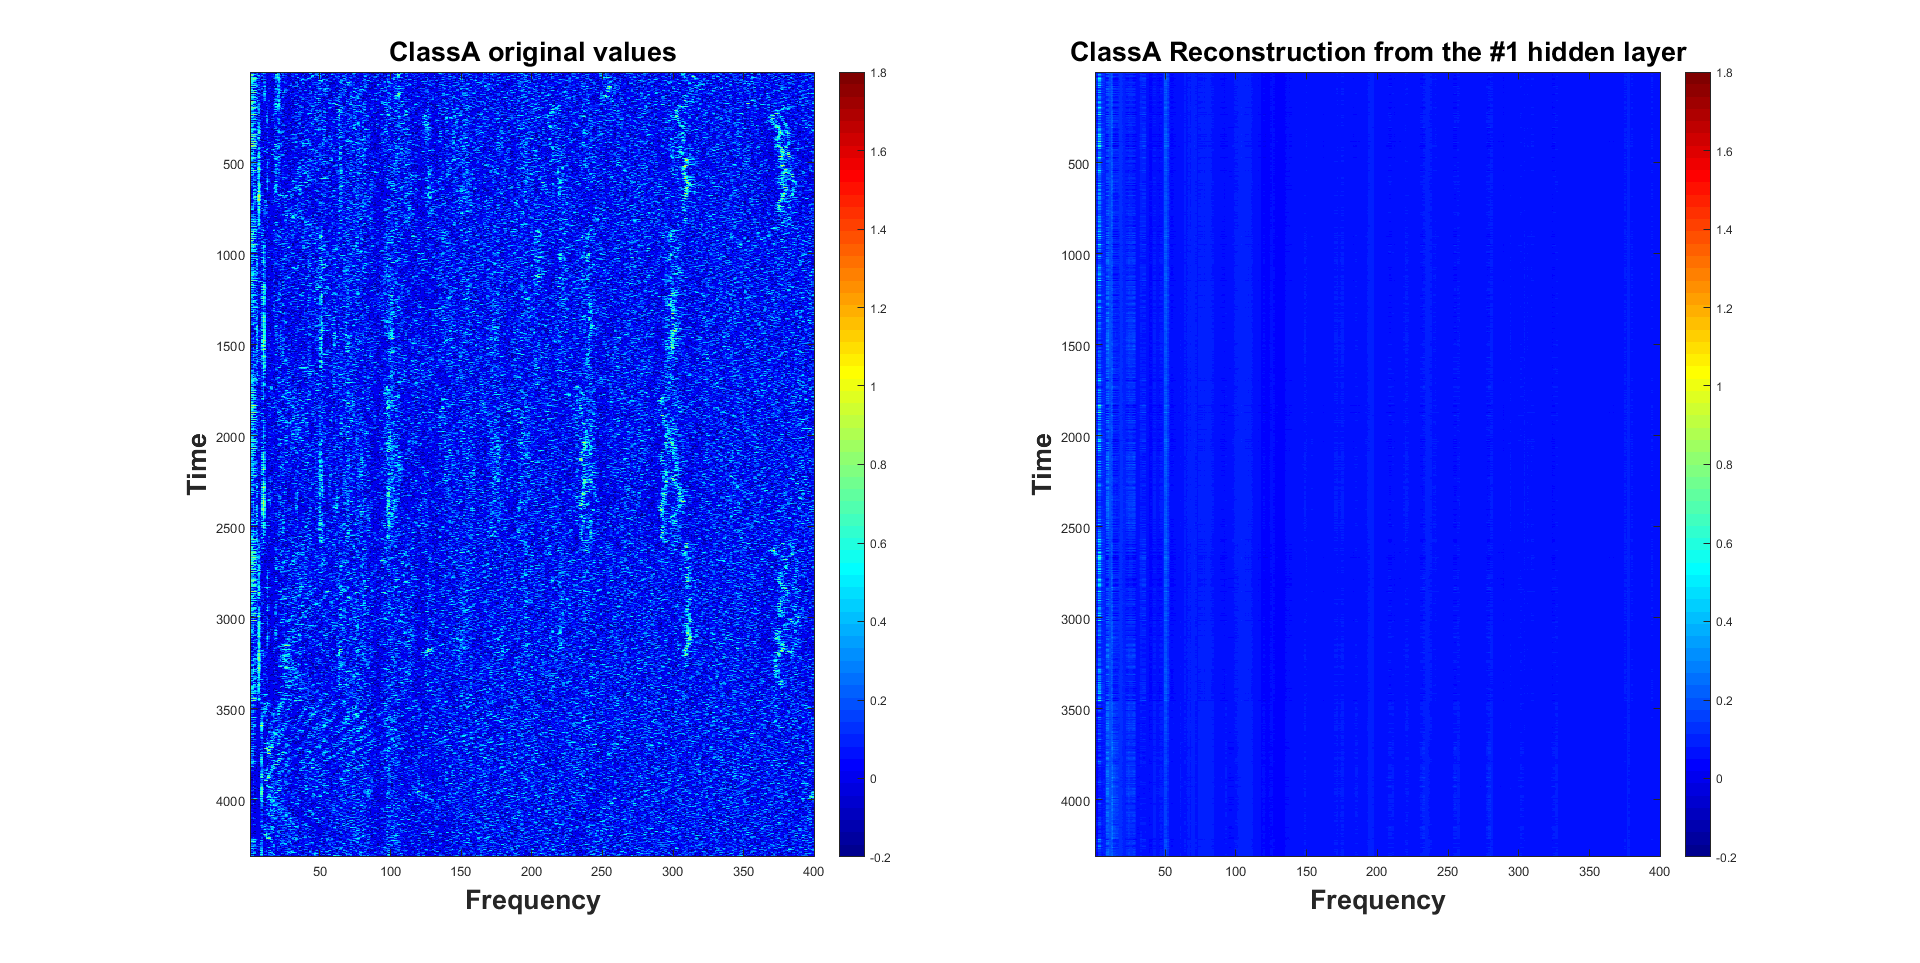
\includegraphics[width=1.3\linewidth]{picts/reconstruction_ClassA_v2_only1st.png}
%		\caption{Classe 1 - Entrada original e reconstrução}
%	\end{figure}
	\begin{figure}[H]
		\hspace{-2cm}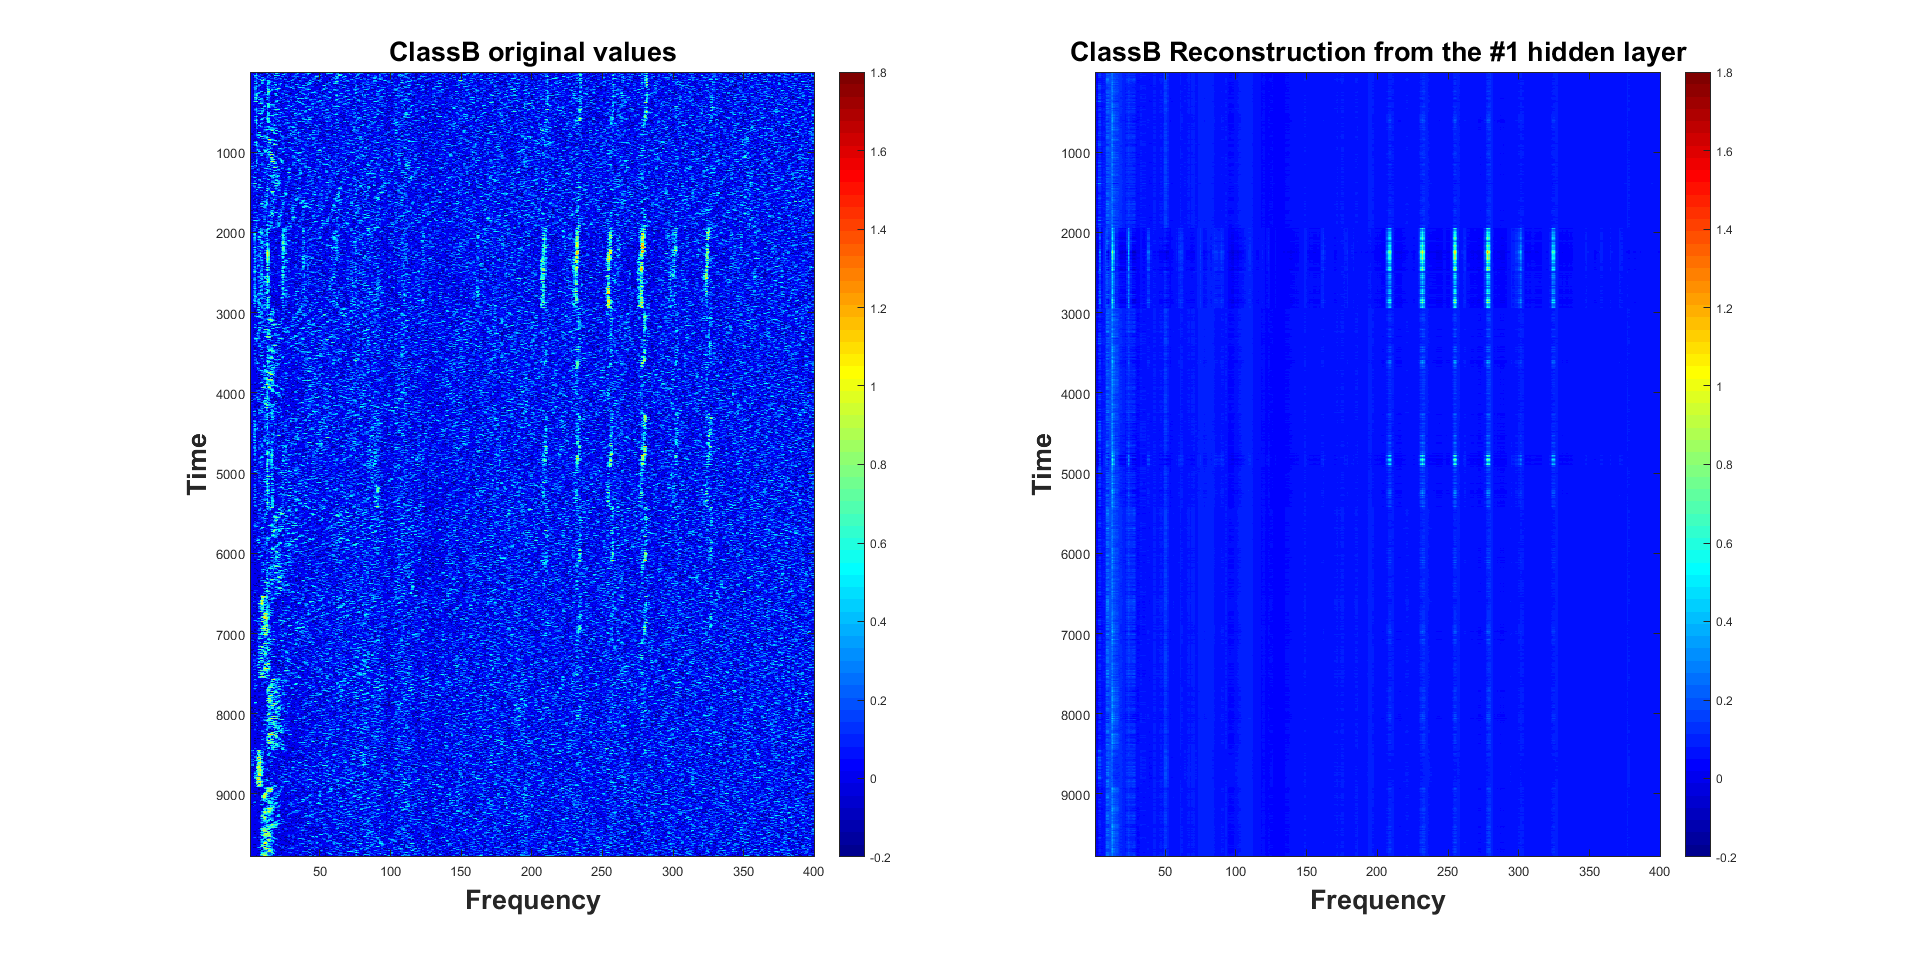
\includegraphics[width=1.3\linewidth]{picts/reconstruction_ClassB_v2_only1st.png}
		\caption{Classe 2 - Entrada original e reconstrução}
	\end{figure}
%	\begin{figure}[H]
%		\hspace{-2cm}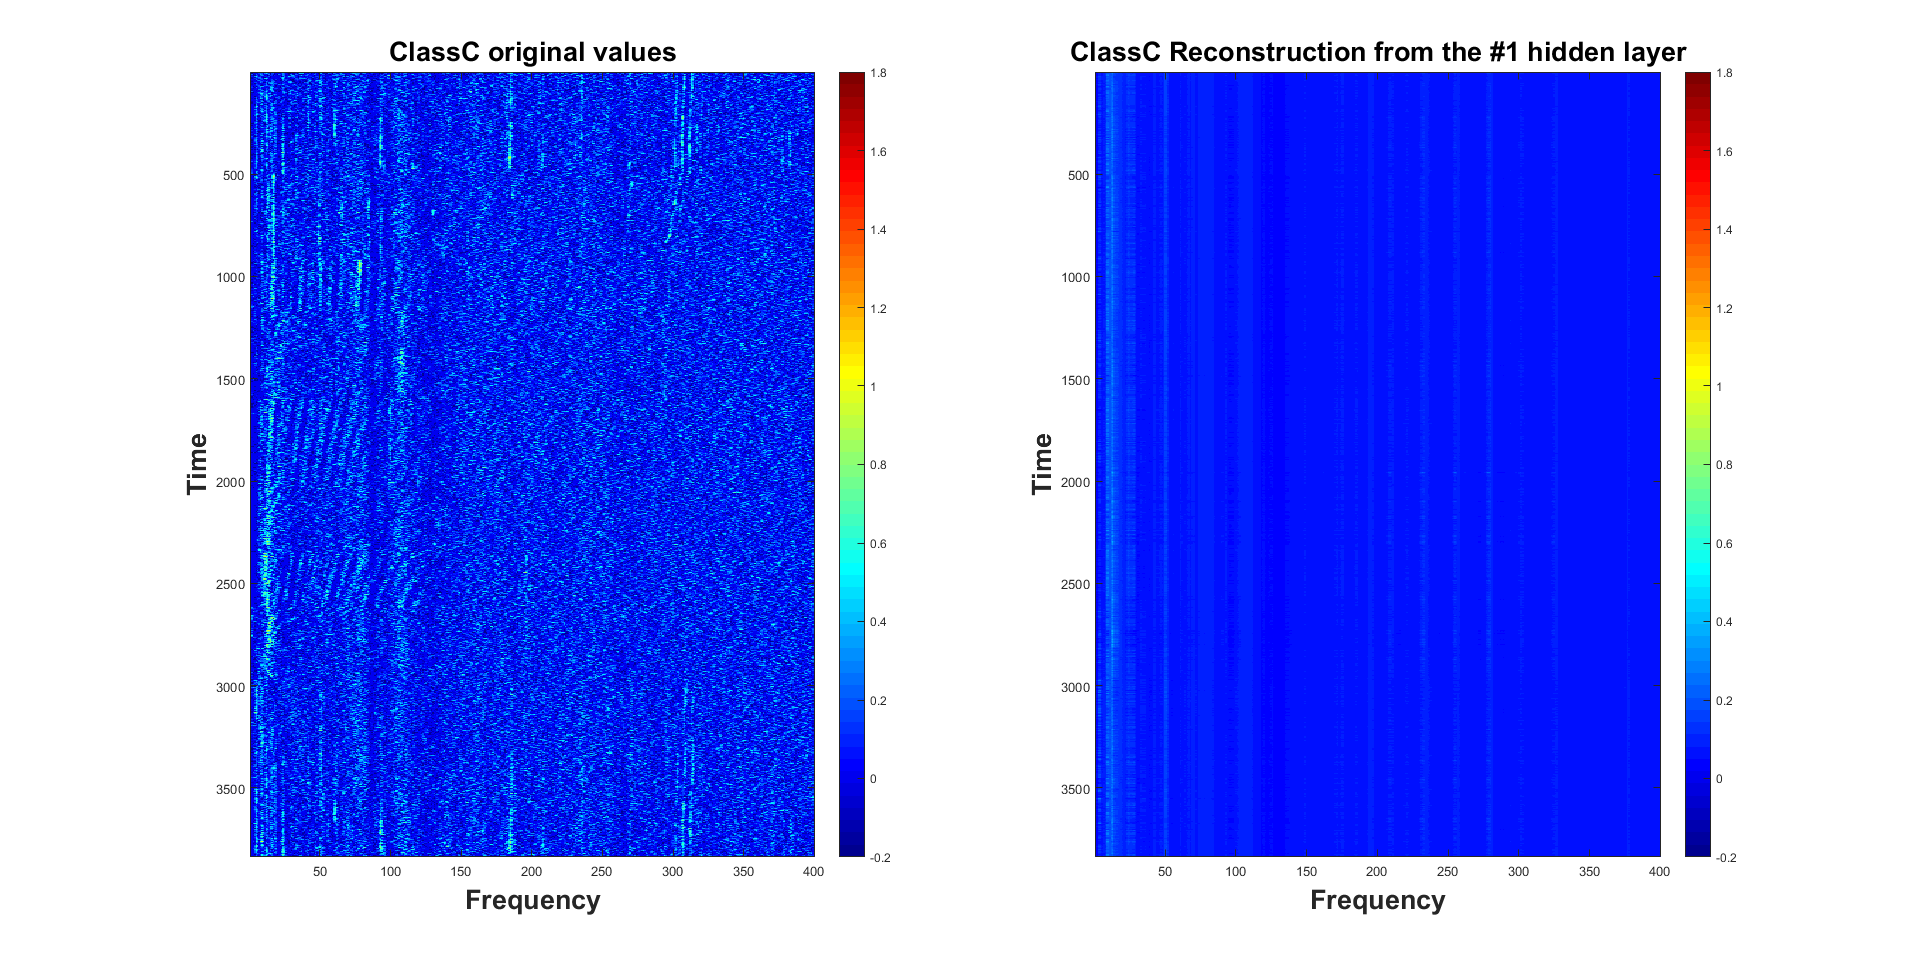
\includegraphics[width=1.3\linewidth]{picts/reconstruction_ClassC_v2_only1st.png}
%		\caption{Classe 3 - Entrada original e reconstrução}
%	\end{figure}
%	\begin{figure}[H]
%		\hspace{-2cm}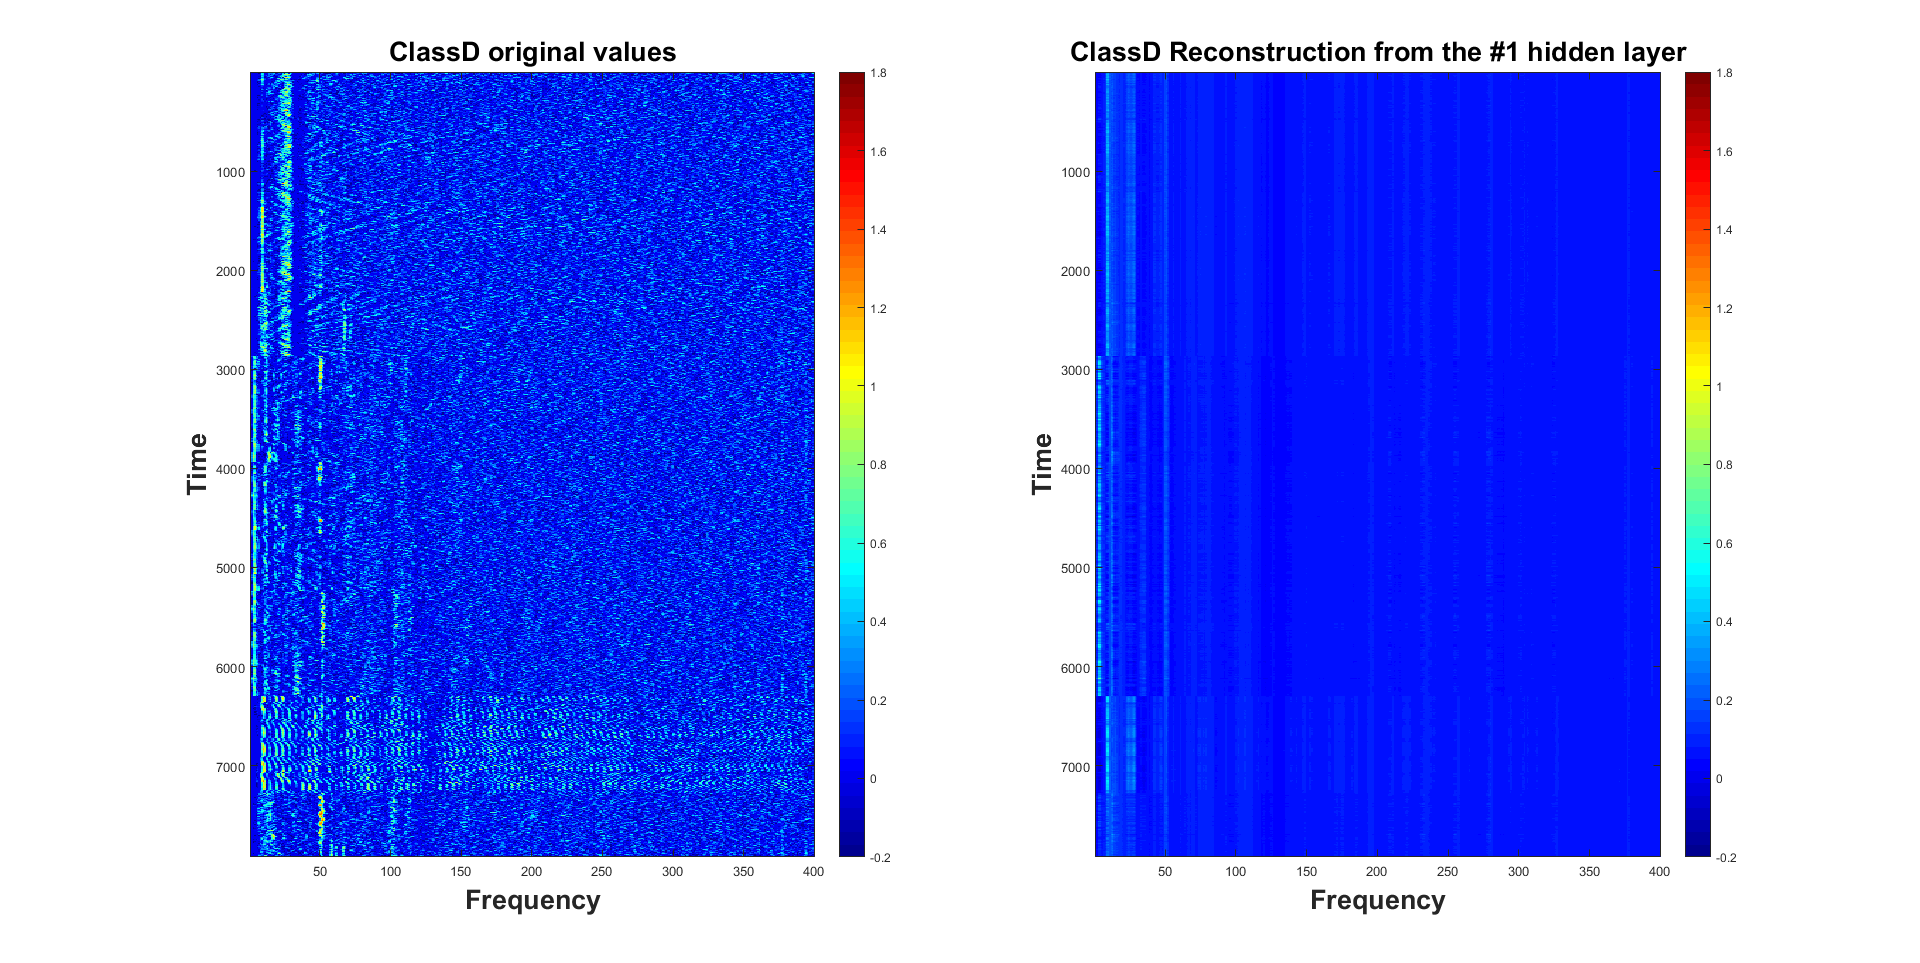
\includegraphics[width=1.3\linewidth]{picts/reconstruction_ClassD_v2_only1st.png}
%		\caption{Classe 4 - Entrada original e reconstrução}
%	\end{figure}
	O gráfico acima mostra um exemplo da tendência do primeiro autoencoder extrair características dos dados de entrada. Para a \textbf{classe 2}, a reconstrução da entrada realçou bins de frequência que estavam bem nítidos na entrada.\\\\
	A seguir, seguem duas matrizes de confusão, que traduzem o desempenho da rede em classificar as entradas com relação aos alvos definidos para cada uma delas:
	\begin{figure}[H]
		\vspace{-4cm}
		\hspace{-5cm}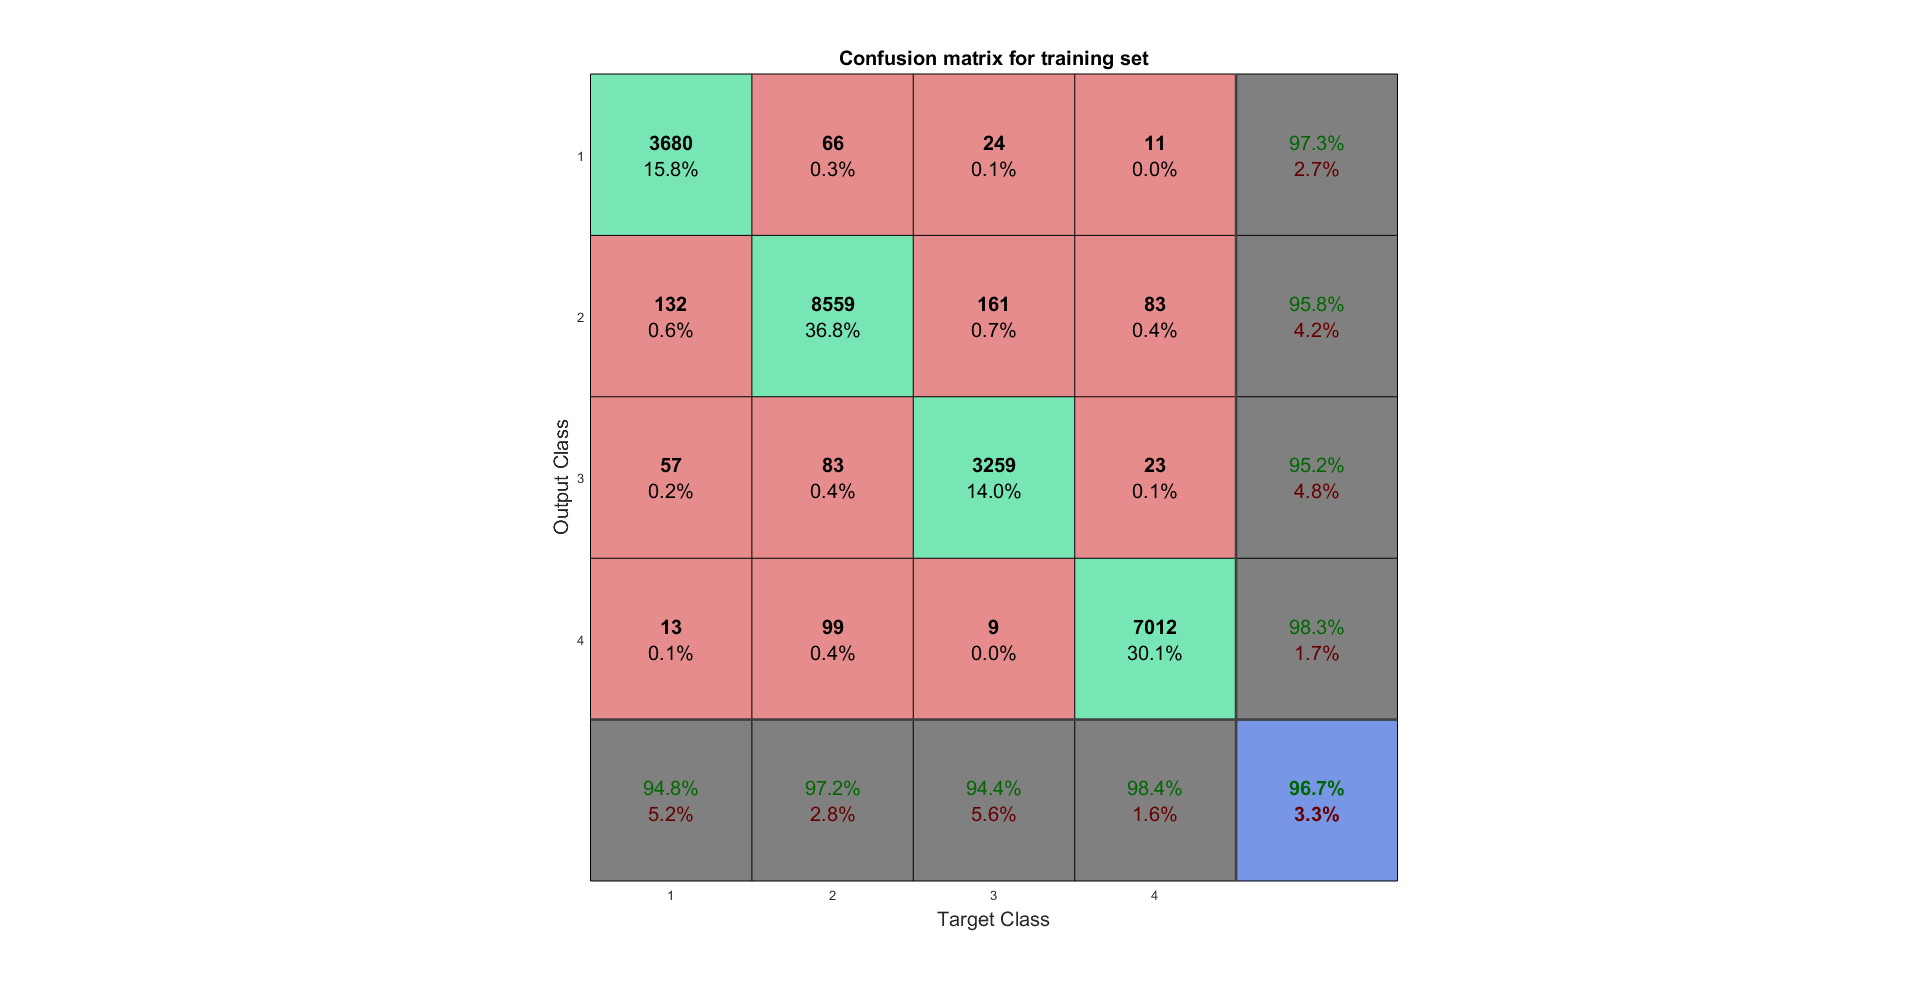
\includegraphics[width=1.8\linewidth]{picts/confusion_train.png}
		\vspace{-1.2cm}\caption{Matriz de confusão para o conjunto de treinamento}
		
		\vspace{0.8cm}
	\end{figure}
	Fazendo uma análise da matriz de confusão acima extraída de eventos do conjunto de treinamento, pode-se observar que os desempenhos por classe ficaram bem próximos entre si:
	\begin{itemize}
		\item 94,8\% dos eventos etiquetados como Classe 1 foram corretamente classificados
		\item 97,2\% dos eventos etiquetados como Classe 2 foram corretamente classificados
		\item 94.4\% dos eventos etiquetados como Classe 3 foram corretamente classificados
		\item 98.4\% dos eventos etiquetados como Classe 4 foram corretamente classificados
	\end{itemize}
	Outro resultado a se avaliar é a Probabilidade de Detecção do classificador:
	\begin{itemize}
		\item 97,3\% dos eventos classificados como Classe 1 eram de fato da Classe 1
		\item 95,8\% dos eventos classificados como Classe 2 eram de fato da Classe 2
		\item 95,2\% dos eventos classificados como Classe 3 eram de fato da Classe 3
		\item 98,3\% dos eventos classificados como Classe 4 eram de fato da Classe 4
	\end{itemize}
	\vspace{0.5cm}
	Além disso, dentre o total de eventos, 96,7\% foram classificados corretamente.

	\begin{figure}[H]
		\vspace{-4cm}
		\hspace{-5cm}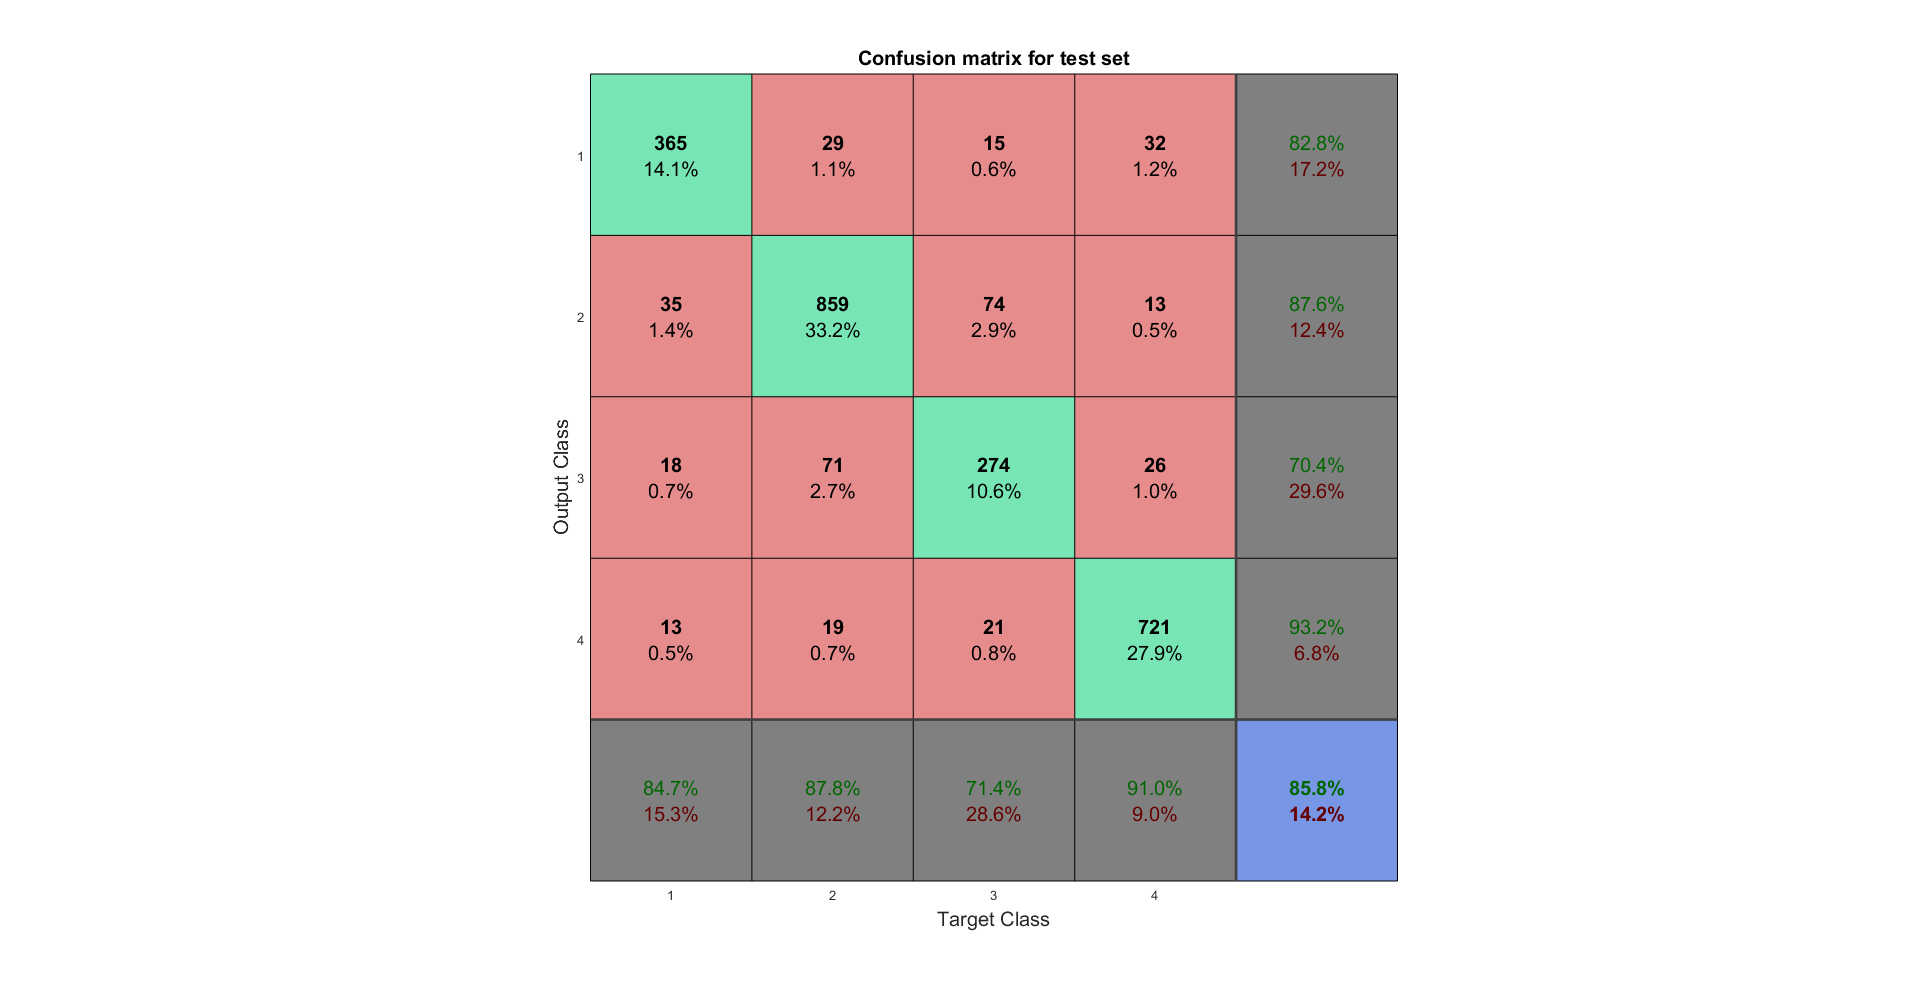
\includegraphics[width=1.8\linewidth]{picts/confusion_test.png}
		\vspace{-1.2cm}\caption{Matriz de confusão para o conjunto de teste}
	\end{figure}
	Analisando da mesma forma os resultados do conjunto de teste, observa-se que o desempenho na classificação da classe 3 foi bem inferior ao das outras classes:
	\begin{itemize}
		\item 84,7\% dos eventos etiquetados como Classe 1 foram corretamente classificados
		\item 87,8\% dos eventos etiquetados como Classe 2 foram corretamente classificados
		\item 71.4\% dos eventos etiquetados como Classe 3 foram corretamente classificados
		\item 91,0\% dos eventos etiquetados como Classe 4 foram corretamente classificados
	\end{itemize}
	Analisando a Probabilidade de Detecção:
	\begin{itemize}
		\item 82,8\% dos eventos classificados como Classe 1 eram de fato da Classe 1
		\item 87,6\% dos eventos classificados como Classe 2 eram de fato da Classe 2
		\item 70,4\% dos eventos classificados como Classe 3 eram de fato da Classe 3
		\item 93,2\% dos eventos classificados como Classe 4 eram de fato da Classe 4
	\end{itemize}
	\vspace{0.5cm}
	Dentre o total de eventos, 85,8\% foram classificados corretamente. A Classe 3 pode estar sendo confundida com outras classes, especialmente a Classe 2, já que 2,9\% dos eventos da Classe 3 foram classificados erroneamente como Classe 2 e, dos eventos classificados como Classe 3, 2,7\% pertenciam à Classe 2.
	
	\begin{figure}[H]
		\hspace{-2.75cm}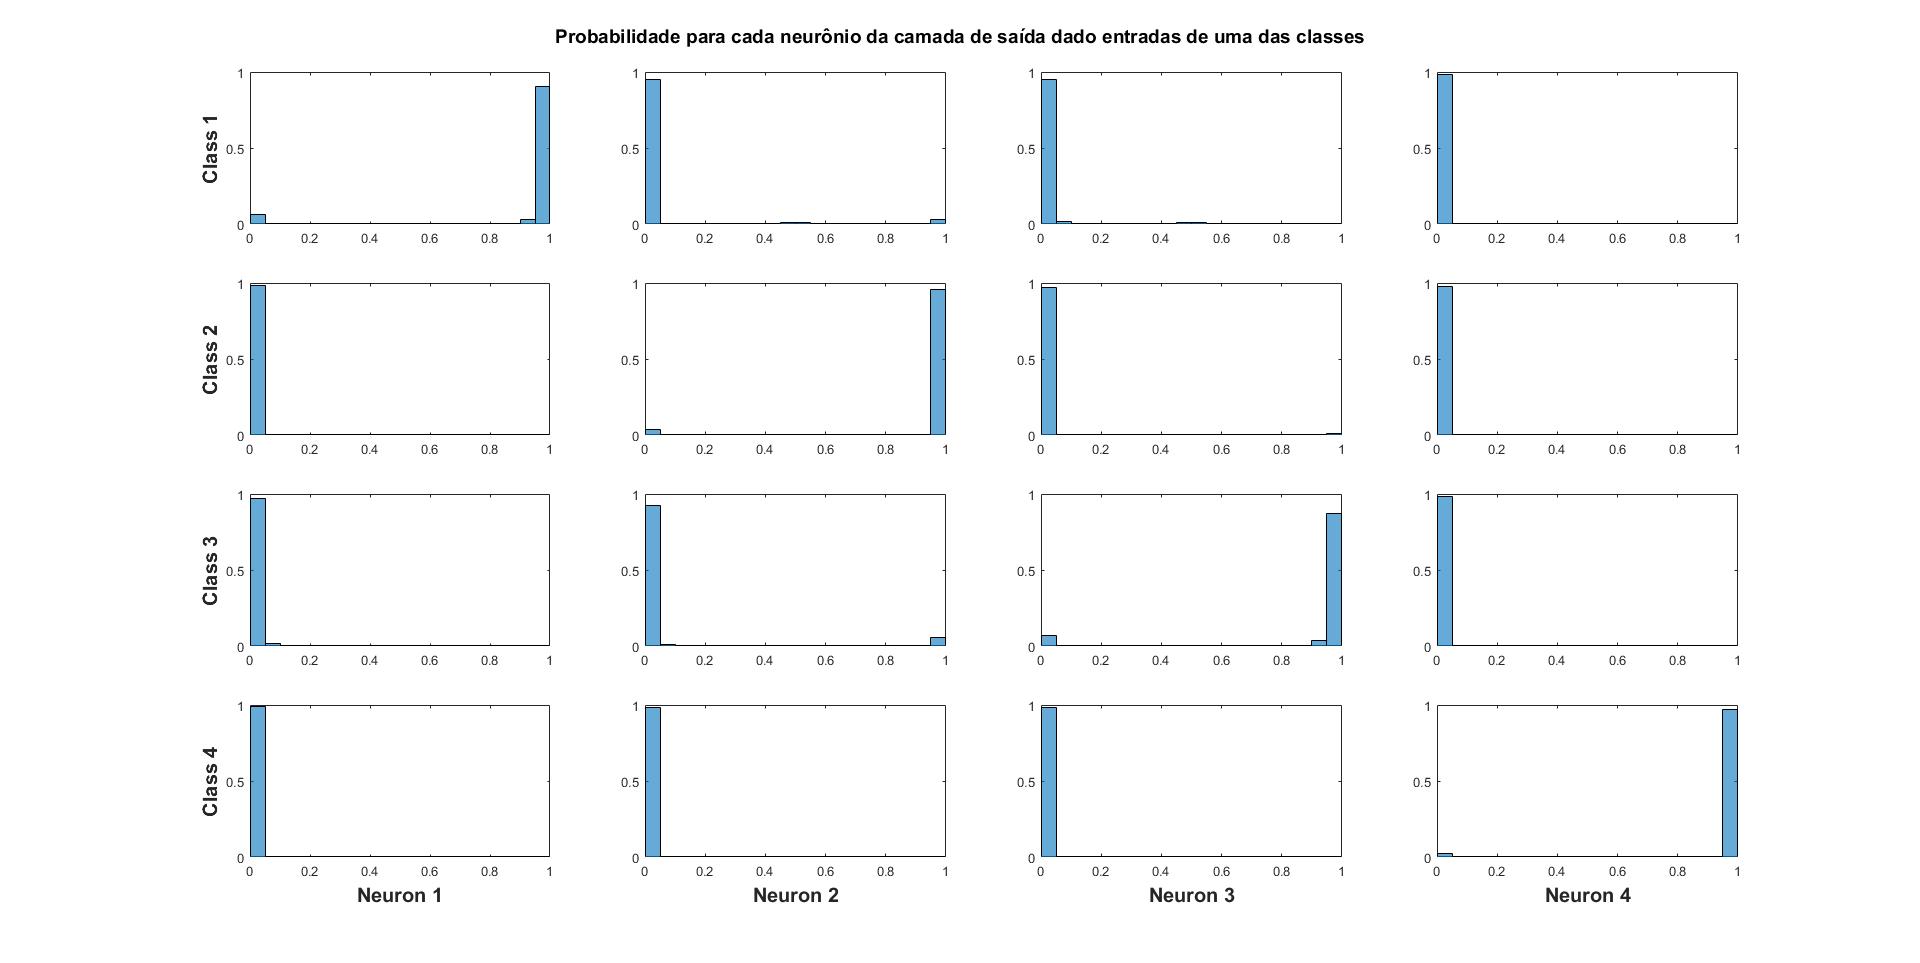
\includegraphics[width=1.4\linewidth]{picts/outputs_16x16}
		\vspace{-1.2cm}\caption{Distribuições na camada de saída por classe e por neurônio}
		\label{fig:outputs_16x16}
	\end{figure}
	\hspace{-0.5cm}Pelo gráfico acima, observamos o comportamento esperado dos neurônios da camada de saída. A distribuição de saída encontra-se saturada nos pontos de treinamento, mostrando que a extração de características (feita pelas camadas mais próximas à entrada) tende a aumentar o poder discriminatório das entradas. \\
	 A etiquetagem dos eventos por classe foi feita de forma que somente um neurônio da saída ficasse ativo para uma classe específica. O neurônio 1 é ativado para eventos da classe 1, o neurônio 2 é ativado para eventos da classe 2 e sucessivamente. Além disso, essas distribuições corroboram com o resultado das matrizes de confusão, pois eventos da classe 3 excitaram o neurônio 2, podendo levar a uma classificação errônea.
	
	\section*{Conclusões}
	Analisando os resultados acima, o \textit{Stacked Autoencoder} obteve um bom desempenho para a classificação dos sinais de navios cedidos pela Marinha e a extração de características da entrada pôde ser confirmada através da reconstrução do primeiro \textit{autoencoder} do SAE. A classe C obteve um desempenho inferior ao das outras, porém o fato das classes não possuírem o mesmo número de eventos pode favorecer o treinamento de uma classe em detrimento de outra.\\\\
	Por fim, mais testes serão realizados para se chegar à melhor estrutura para o SAE e para conseguir uma extração de características da entrada que leve a um melhor treinamento de classificação.
	
	\begin{thebibliography}{9}
		\bibitem{layer-wise}
		Yoshua Bengio, Pascal Lamblin, Dan Popovici e Hugo Larochelle (2006).
		Greedy Layer-Wise Training of Deep Networks.
		\textit{Dept.IRO, Université de Montréal}.
		
		\bibitem{sae-representation}
		Pascal Vincent, Hugo Larochelle, Isabelle Lajoie, Yoshua Bengio e Pierre-Antoine Manzagol (2010).
		Stacked Denoising Autoencoders: Learning Useful Representations in a Deep Network with a Local Denoising Criterion.
		\textit{Journal of Machine Learning}
		
		\bibitem{tutorial} 
		Yoshua Bengio, Yann LeCun (2009). 
		Tutorial: Learning Deep Architectures. 
		\textit{ICML Workshop on Learning Feature Hierarchies}.
		
		\bibitem{dimensionality}
		G.E. Hinton, R.R. Salakhutdinov (2006).
		Reducing the Dimensionality of Data with Neural Networks
		\textit{Science, 28 Jul 2006}
		
		\bibitem{sae-stanford}
		http://ufldl.stanford.edu/wiki/index.php/Stacked\_Autoencoders

		\bibitem{william1_ref}
		Soares-Filho W., J. Manoel de Seixas, and L. Pereira Caloba, Principal component analysis for classifying passive sonar signals, ISCAS, vol. 3, pp. 592–595, May 2001.
		
		\bibitem{william2_ref}
		Soares-Filho W., J. Manoel de Seixas, and L. Pereira Caloba, Enlarging neural class detection capacity in passive sonar system, Proc. IEEE Int. Symp. Circuits and Systems, pp. 105-108, May 2002.
		
		\bibitem{lofargram_ref}
		Di Martino, J.C.; Haton, J.P.; Laporte, A., Lofargram line tracking by multistage decisionprocess. IEEE International Conference on Acoustics, Speech, and Signal Processing, Minneapolis, USA, vol. 1, pp. 27-30 April, 1993.

		
	\end{thebibliography}
	
	\chapter*{Comentários finais}
		\section*{Avaliação feita pelo bolsista}
		Sem dúvida, essa iniciação científica só me acrescentou coisas boas. Estou estudando um assunto pelo qual me interesso muito e que está em alta, conheci pessoas brilhantes no ambiente de trabalho e amadureci muito no âmbito de pesquisa. Pretendo continuar no projeto buscando resultados ainda melhores e só tenho a agradecer ao professor Seixas e a um de seus alunos de doutorado, Natanael Júnior, que estão me auxiliando muito nesse projeto.
		
		
\end{document}          
